\documentclass[10pt,a4paper]{article}
\usepackage[top=0.75in, bottom=1in]{geometry}
\usepackage[latin1]{inputenc}
\usepackage{amsmath}
\usepackage{amsfonts}
\usepackage{amssymb}
\usepackage{graphicx}
\usepackage{fancyhdr}
\usepackage{mathrsfs}
\usepackage[mathscr]{eucal}
\usepackage{tikz}
\usetikzlibrary{patterns}
\usepackage{algpseudocode}
\usepackage[makeroom]{cancel}
\usepackage{enumerate}
\usepackage{enumitem}  
\usepackage{subfigure}
\usepackage{chemfig}
\usepackage{textcomp}
\usepackage{siunitx}
\newcommand{\indentitem}{\setlength\itemindent{25pt}}
\newcommand{\jw}{j\omega}
\newcommand{\tab}{\hspace*{5mm}}
\newcommand{\tr}{\textrm}
%\author{Ethan Morse}
\title{ECEN 664 Homework 5: Deposition}
\date{Due: 21 November 2019}

\pagestyle{fancy}
%\rhead{Ethan Morse ECEN 664 Homework 5}
\headheight 8mm

\begin{document}
	%
	\maketitle

	{\flushleft {\bf Problem 1: Deposition: CVD. (30 points)}}
	
	The following reaction is used to deposit polysilicon by CVD process from SiCl4. The
	concentration of SiCl4 is $C_{G}$ = 4.0e16 molecules/cm3 and gas transfer coefficient is
	$h_{G}$ = 2.55 cm/sec. Estimate film deposition rate. Assume that the growth process is mass transfer limited. Atomic density of polysilicon is $\rho$ = 5.0e22 atoms/cm3.
	
	The thickness growth rate is given by:
	\[\dfrac{dy}{dt} = \dfrac{1}{\dfrac{1}{k_{S}} + \dfrac{1}{h_{G}}} \dfrac{C_{G}}{\rho}\]
	
	Because the is mass transfer limited, $k_{S}$ can be considered negligible when compared to $h_{G}$. Thus, the thickness growth rate becomes:
	\[\dfrac{dy}{dt} = \dfrac{C_{G}h_{G}}{\rho}\]
	
	Substitute values:
	\[\dfrac{dy}{dt} = \dfrac{(4 \times 10^{16})(2.55)}{(5 \times 10^{22})}\]
	\[\boxed{\dfrac{dy}{dt} = \SI{2.04}{\micro\meter/\second}}\] \bigbreak
	
	\clearpage
	
	{\flushleft {\bf Problem 2: Evaporation: Shadow masking. (30 points)}}
	
	Assume that the evaporation source is very far from wafer and the evaporation flux is
	uniform and parallel. If the deposition rate is 100 nm/min, sketch the cross-sectional
	profile of film over the SiO2 and silicon after 1 min and 2 minutes.
	
	\vspace*{10mm}

	\begin{figure}[h]
		\centering
		\includegraphics[scale=0.58]{ecen664_hw5_fig1}
		\caption{Intitial cross-sectional profile}
	\end{figure}

	\vspace*{20mm}

	\begin{figure}[h]
		\centering
		
		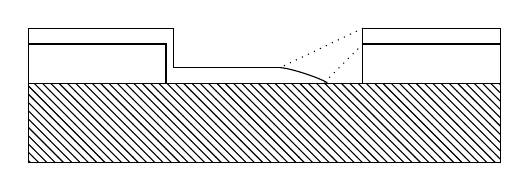
\begin{tikzpicture}
		
		\draw[pattern = north west lines] (0,0) -- (0,1) -- (6,1) -- (6,0) -- (0,0);
		
		\draw (0,1) -- (0,1.5) -- (1.75,1.5) -- (1.75,1) -- (4.25,1) -- (4.25,1.5) -- (6,1.5) -- (6,1) -- (0,1);
		
		\draw (0,1.5) -- (0,1.7) -- (1.84,1.7) -- (1.84,1.2);
		
		\draw (4.25,1.5) -- (4.25,1.7) -- (6,1.7) -- (6,1.5) -- (4.25, 1.5);
		
		\draw (1.84,1.2) -- (3.2,1.2);
		\draw (3.2,1.2) to[out=-5,in=-10] (3.75,1);
		
		\draw[dotted] (4.25,1.5) -- (3.75,1);
		\draw[dotted] (4.25,1.7) -- (3.2,1.2);
		
		\end{tikzpicture}
		
		\caption{Cross-sectional profile after 1 min deposition (not drawn to scale)}
		
	\end{figure}

	\vspace*{20mm}
	
	\begin{figure}[h]
		\centering
		
		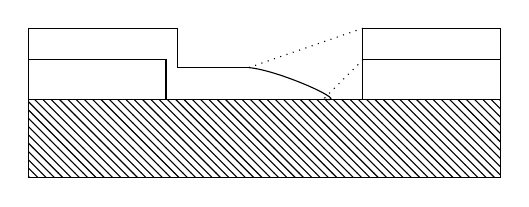
\begin{tikzpicture}
		
		\draw[pattern = north west lines] (0,0) -- (0,1) -- (6,1) -- (6,0) -- (0,0);

		\draw (0,1) -- (0,1.5) -- (1.75,1.5) -- (1.75,1) -- (4.25,1) -- (4.25,1.5) -- (6,1.5) -- (6,1) -- (0,1);
		
		\draw (0,1.5) -- (0,1.9) -- (1.9,1.9) -- (1.9,1.4);
		
		\draw (4.25,1.5) -- (4.25,1.9) -- (6,1.9) -- (6,1.5) -- (4.25, 1.5);
		
		\draw (1.9,1.4) -- (2.8,1.4);
		\draw (2.8,1.4) to[out=-5,in=-10] (3.75,1);
		
		\draw[dotted] (4.25,1.5) -- (3.75,1);
		\draw[dotted] (4.25,1.9) -- (2.8,1.4);
		
		\end{tikzpicture}
		
		\caption{Cross-sectional profile after 2 min deposition (not drawn to scale)}
	\end{figure}


\newpage

\[\sum_{i = 0}^{n} i^{3}\]
	
%\[\sum\nolimits_{i = 0}^{n} i^{3}\]










\end{document}